\section{Introduction}
\begin{comment}
[talk about what LLM agents do now, therefore motivated the necessaty of memory] LLM agents that are capable of autonomous task completion requires agents to persist, adapt, and interact coherently over time. From this goal, memory where history is stored, managed, and updated works as a core function in autonomous agents. 
[provide background on how memory is usually implemented in agents, which lead to the designs of existing evaluation benchmarks] Current LLM agents instantiate the memory function in two ways: 
(1) pre-appending (raw) history previous steps as a static long context before input using the \textit{internal} long-context capacity of LLMs; 
(2) coupling the agent with \textit{external} memory systems which dynamically manage the history and provide useful content. 
[draw a conclusion that currently there are too many memory works] Currently, efforts to enlarge LLM's effective modeling context window and design memory systems are emerging.

[let people think about the phenomenon that memory evaluation is naive and shallow compared to the effort spent to design memory system] However, evaluations are trivial and scared compared to the rapid development of proposing memory systems. 
[why memory benchmark is shallow: no environment and agency] Existing memory evaluation benchmarks only focused on static user-agent dialog and evaluates using long-context question answering or summarization tasks, such as LOCOMO or LongMemBench. As a result, the LLM agent that are evaluated is usually a chatbot -- no agency and no interaction with the environment over time.
[a result of shallow memory benchmark] An evidence is current memory systems usually achieve more than 90\% accuracy in LOCOMO. 
[why agent benchmark is shallow: no long-term memory and memory system evaluation, only single session] Conversely, agent benchmarks such as webarena or wind2web explicitly evaluate the agency of LLM agents over tasks. As finishing a task usually requires the agent, they are also claimed to evaluate long-horizon agent memorization capacity. However, they usually append flat reasoning trace in the context window at each step, only evaluate over single task, where the history in a single episode is effective as a short working memory to solve those single session agent tasks.  
[a result of shallow agent benchmark] However, real-world agent tasks usually require maintaining a persistent, latent task state that is incrementally constructed through interaction. Early decisions introduce constraints—such as compatibility requirements, shared preferences, or intermediate results—that are not restated explicitly but must be remembered and correctly reused to ensure future actions remain valid.

[From now talks about our work. start from our vision or what we believe] We argue that memory as a core competence of LLM agents should be evaluated by agentic tasks in a interactive environments, messuring its capacity to track stateness of environment dynamics over time and evaluated by the goal completion with the help of memory component. 
We argue that memory can only be meaningfully evaluated in agents when it functions as a persistent task-state representation captured through interactions between agent to memory, taking memory-conditioned actions, and get feedback from the environment for the next step, in the other words, to be evaluated in the agent Memory-Action-Environment loops.
In many practical tasks, early interactions introduce latent constraints—such as compatibility requirements, shared preferences, or intermediate reasoning results—that are not restated by the environment but must be retained and correctly applied in later decisions. Evaluating memory in such settings requires tasks that span multiple sessions and exhibit explicit dependency across subtasks.


[What we designed in this work and compared with other benchmarks] To this end, we introduce MemArena, a unified evaluation gym for benchmarking the helpfulness of agent memory in multi-session memory–action–environment loops. 
MemAct Arena consists of agentic tasks with interdependent subtasks, manually crafted by human experts, where future queries are usually the follow-ups and later actions are underspecified unless agents correctly track and reuse task-relevant information from prior interactions.
We enable standardized multi-session evaluation across four test scenarios to test how memory could help when doing web navigation and shopping over a bundle of dependent products, preference-constrained travel planning, compositional information searching, and sequential formal reasoning over math or physical problems. 
Each multi-session task has many interdependent sub-tasks, long-horizon with more than XX action steps, and long reasoning trace with XXX tokens. 
Table 1 compares MemArena with previous relevant benchmarks. 

[what we found in this work] We test three categories of main-stream long agents in MemArena, including long-context agents, agents coupled with memory systems, or agents augmented with RAG systems. 
Results shows agents that even though achieves 90\% accuracy on LOCOMO or LongMemBench, yeilds low success rate when really doing agentic tasks, indicating
task completion under the current SOTA memory systems still is challenging or requires an improved competence to work together,
and the gap between existing long-context evaluation benchmarks and real agent memory evaluation protocal with agentic tasks, 
calling for more rigious long-horizon agent memory evaluation works like us. 

\end{comment}

\begin{table*}[ht]
\centering
\resizebox{\textwidth}{!}{%
\begin{tabular}{@{}ccccccccc@{}}
\toprule
 &
  \multicolumn{3}{c}{\textbf{Memory-Agent-Env. Loops}} &
   &
   &
  \multicolumn{3}{c}{\textbf{Task Settings}} \\ \cmidrule(lr){2-4}\cmidrule(lr){5-9}
\textbf{Benchmark} &
  \textbf{\begin{tabular}[c]{@{}c@{}}Memory \\ Eval.\end{tabular}} &
  \textbf{\begin{tabular}[c]{@{}c@{}}Agentic\\ Actions\end{tabular}} &
  \textbf{\begin{tabular}[c]{@{}c@{}}Env.\\ Feedback\end{tabular}} &
  \textbf{\begin{tabular}[c]{@{}c@{}}Multi-Sess.\\ Tasks\end{tabular}} &
  \textbf{\begin{tabular}[c]{@{}c@{}}Interdep.\\ ST\end{tabular}} &
  \textbf{\begin{tabular}[c]{@{}c@{}}\# T\\ (\# Q)\end{tabular}} &
  \textbf{\begin{tabular}[c]{@{}c@{}}\# Interdep. \\ ST\end{tabular}} &
  \textbf{\#S} \\ \midrule
LOCOMO~\cite{maharana2024evaluating} &
  \cmark &
  \xmark &
  \xmark &
  \cmark &
  \xmark &
  7512 &
  1 &
  \multirow{4}{*}{N/A$^1$} \\
LongMemEval~\citep{wulongmemeval} &
  \cmark &
  \xmark &
  \xmark &
  \cmark &
  \xmark &
  500 &
  1 &
   \\
MemoryAgentBench~\citep{hu2025evaluating} &
  \cmark &
  \xmark &
  \xmark &
  \cmark &
  \xmark &
  2k &
  1 &
   \\
MemoryBench~\cite{ai2025memorybench} &
  \cmark &
  \xmark &
  \xmark &
  \cmark &
  \xmark &
  778 &
  1 &
   \\ \midrule
WebArena~\citep{zhouwebarena}&
  \xmark &
  \cmark &
  \cmark &
  \xmark &
  \xmark &
  812 &
  1 &
  13.3 \\
WebShop\citep{yao2022webshop} &
  \xmark &
  \cmark &
  \cmark &
  \xmark &
  \xmark &
  200 &
  1 &
  7.3 \\
VeriGUI~\citep{liu2025verigui} &
  \xmark &
  \cmark &
  \cmark &
  \cmark &
  \xmark &
  130 &
  4.5 &
  214 \\
Evo-Memory~\citep{wei2025evo} &
  \cmark &
  \cmark &
  \cmark &
  \cmark &
  \xmark &
  N/A$^2$ &
  N/A$^2$ &
  N/A$^2$ \\
  AgencyBench~\citep{li2026agencybench} &
  \xmark &
  \cmark &
  \cmark &
  \cmark &
  \cmark &
   138 &
  $4.31^3$ &
  90 \\
   \midrule
\textbf{\ours} &
  \cmark &
  \cmark &
  \cmark &
  \cmark &
  \cmark &
  766 &
  6.9 &
  57 \\ \bottomrule
\end{tabular}%
}
\vspace{0.5em}
\caption{We compare benchmarks along key dimensions: if the benchmark evaluates different memory mechanism, if it evaluates agent actions, and if it involves environment feedbacks in memory–agent–environment loops. We also compare their evaluation task settings and scales. (Notations: \textbf{T.}: tasks;\textbf{ ST.}: subtasks; \textbf{Env.}: environment; \textbf{Interdep.}: interdependent; \textbf{S.}: Steps, \textbf{Q}: Queries). Green checkmarks indicate supported features; red crosses indicate unsupported features.
\textbf{Note 1:} These benchmarks use long-context conversational QA tasks without agentic actions; thus, the number of action steps is Not Applicable (N/A).
\textbf{Note 2:} Evo-Memory constructs a multi-session setting by executing \textit{independent} tasks from existing single-session agent benchmarks sequentially. Because these tasks are \textit{directly reused}, there is no explicit subtask-level dependency or cross-session causal structure enforced. So the number of tasks, interdependent subtasks, and per-task action steps cannot be meaningfully defined or aggregated. We marked them as N/A. \textbf{Note 3:} Computed from the official AgencyBench-v2 release.
}
\label{tab:benchmark-positioning}
\vspace{-15pt}
\end{table*}


% == version 2==

Large language model (LLM) agents have two complementary core capabilities: the ability to memorize task-relevant knowledge over time (\emph{memorization}) and the ability to act through interaction with an environment (\emph{action}) \cite{hu2025evaluating}. However, existing evaluations of LLM agents with memory typically isolate and assess only one aspect.
% one of these dimensions.
\begin{figure}[t]
    \centering
    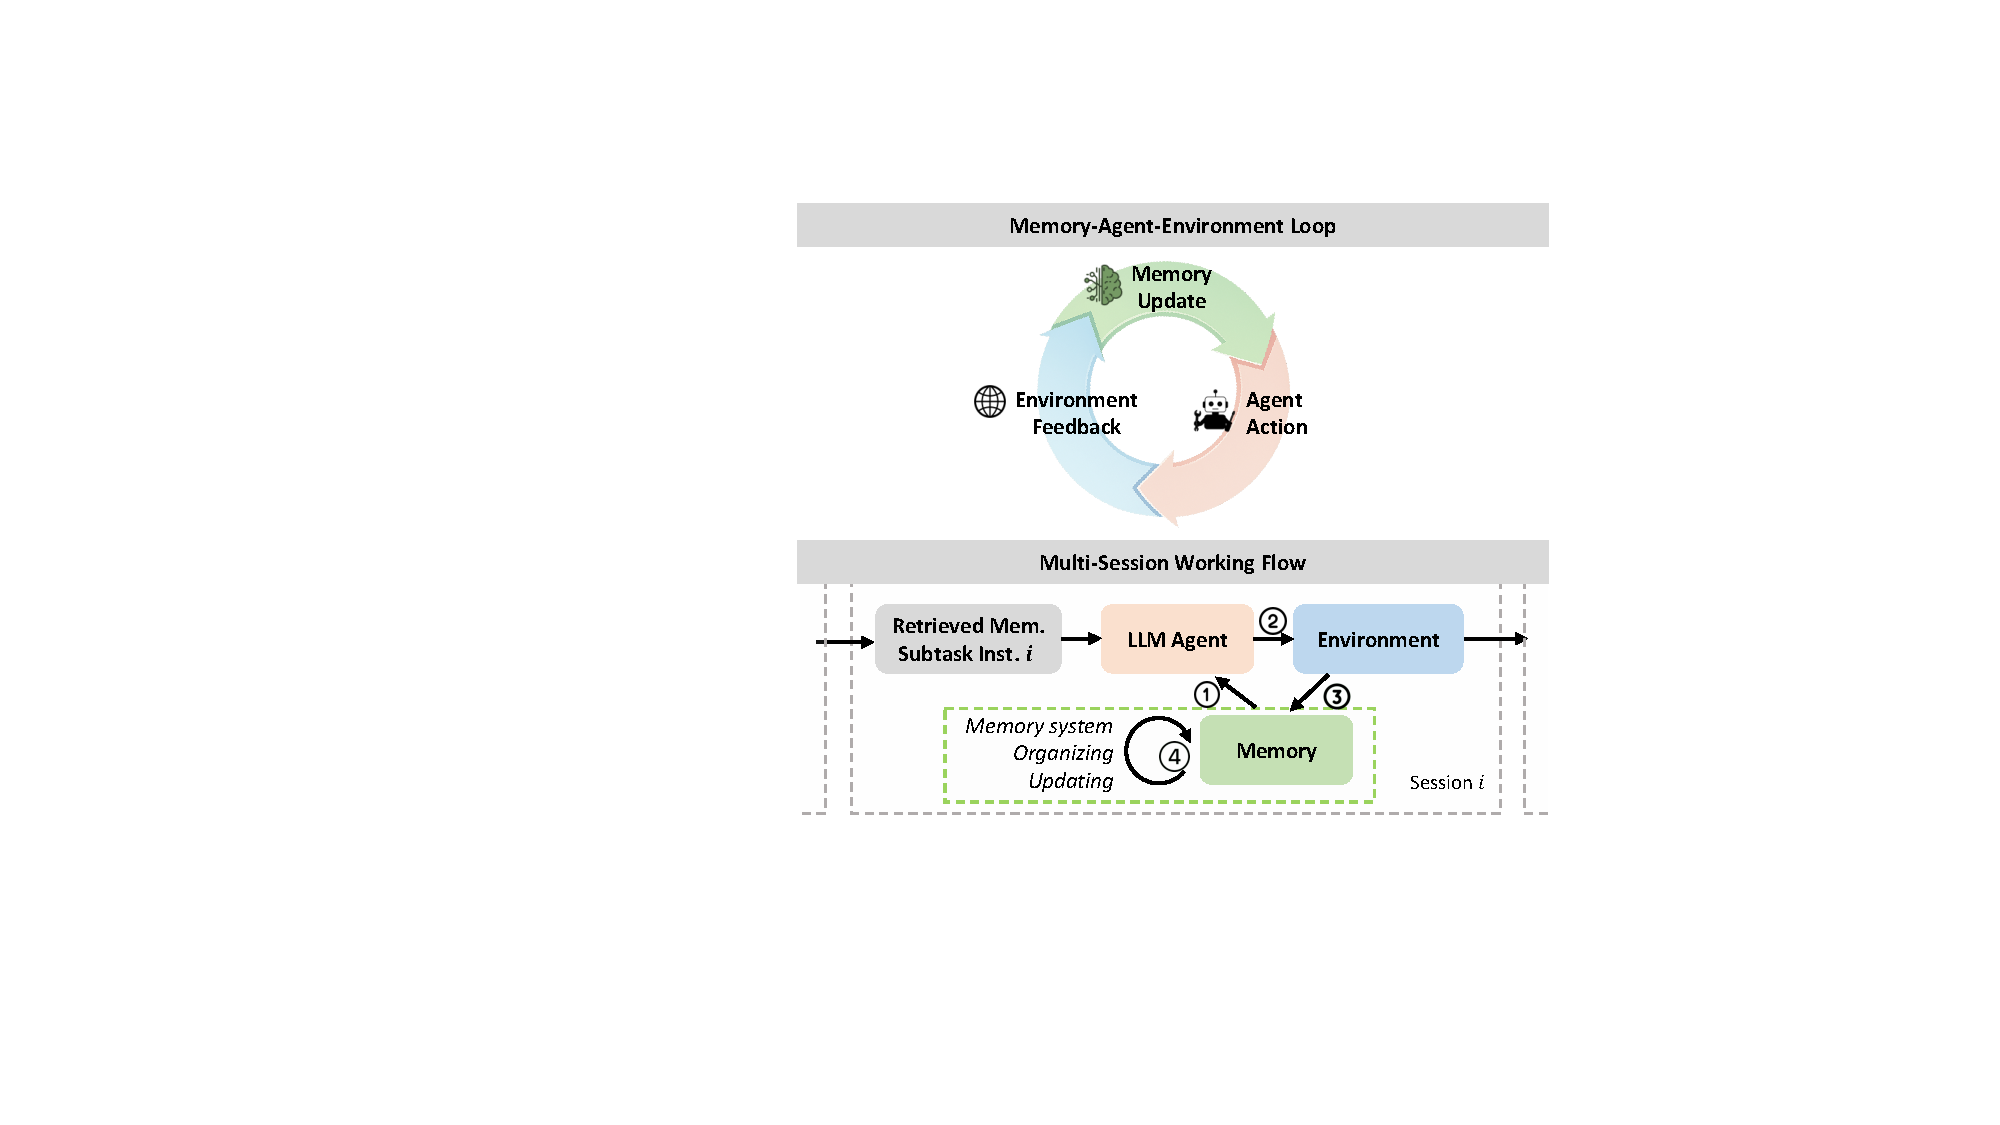
\includegraphics[width=\linewidth]{figs/teaser_memoryarena.pdf}
    \caption{\ours Evaluates agents with Memory with multi-session tasks in a Memory-Agent-Environment Loop. }
    \label{fig:teaser}
    \vspace{-15pt}
\end{figure}
The first class of benchmarks focuses on evaluating \textit{memorization} 
% memory benchmarks primarily evaluate \textit{memorization} 
through recall or retrieval over static long-context inputs in question answering or summarization settings ~\cite{wulongmemeval,zhong2024memorybank,maharana2024evaluating,hu2025evaluating}, including benchmarks such as LoCoMo~\cite{maharana2024evaluating} and LongMemEval~\cite{wulongmemeval}. In these setups, agents are required to memorize provided conversations or text chunks, and are evaluated on whether they can recall specific information through downstream QA tasks. However, despite being effective at measuring factual recall, such benchmarks do not involve agentic decision-making, environment dynamics, or action-dependent consequences. As a result, although contemporary memory systems achieve near-saturated performance on these benchmarks, it remains unclear whether such gains meaningfully translate to improved performance for LLM agents operating in goal-driven, interactive settings.

In contrast, the second class of benchmarks~\cite{yao2022webshop,zhouwebarena,deng2023mind2web}, such as SWE-Bench~\citep{jimenez2023swe} and WebArena~\cite{zhouwebarena}, primarily evaluate \textit{action} by placing agents in dynamic environments, but are typically confined to a single session. In these settings, the previous interaction history is treated as flat context whenever it fits within the model’s context window, so information beyond short-term working memory is not causally required. 
% However, in practical tasks, early interactions introduce latent constraints, such as compatibility requirements, shared preferences, or intermediate reasoning results, that are not restated by the environment but must be retained and correctly applied in later decisions. Evaluating memory in such settings requires tasks that span multiple sessions and exhibit explicit dependency across sub-tasks.
However, in practical tasks, early interactions often introduce latent constraints, including compatibility requirements, shared preferences, and intermediate reasoning outcomes, that are not explicitly restated by the environment yet must be preserved and applied in subsequent decisions. As a result, success in these benchmarks does not reliably reflect an agent’s ability to retain and utilize information over extended horizons.

% We argue that agent memory should be evaluated by treating memorization and action as inseparable components. This requires assessing memory in the full process of a loop where actions induce environment feedback, feedback updates memory, and memory conditions subsequent action selection across multi-session task execution, i.e., within \textit{Action–Feedback–Memorization loops} that span multiple episodes or sessions. In such settings, task success critically depends on correctly retaining and reusing information acquired in earlier sessions.


We argue that agent memory should be evaluated by treating memorization and action as inseparable components of agentic behavior. This requires assessing memory within a full interaction process, in which actions elicit environment feedback, feedback updates memory, and memory in turn conditions subsequent action selection across multi-session task execution. We refer to this process as a \textit{Memory-Agent-Environment loop}, which unfolds over multiple episodes or sessions. In such settings, task success critically depends on an agent’s ability to retain and correctly reuse information acquired in earlier interactions.

To this end,  we introduce \ours, a unified evaluation gym for benchmarking the usefulness of agent memory using \textbf{multi-session}, \textbf{interdependent agentic tasks}. \ours consists of human-crafted tasks with interdependent subtasks, where later actions are underspecified unless agents correctly track task-relevant information from prior sessions. We instantiate \ours across four domains, including \textit{(1) bundled web shopping}, \textit{(2) preference-constrained group travel planning}, \textit{(3) progressive information searching}, and \textit{(4) sequential formal reasoning} over math and physical problems. Each task spans long horizons (with an average of 57 action steps) and produces extended reasoning traces with more than 40k tokens. Table~\ref{tab:benchmark-positioning} compares \ours with existing memory and agent benchmarks along key dimensions.

%\ours supports various classes of state-of-the-art agents, including long-context agents, agents augmented with retrieval-augmented generation (RAG) systems, and agents coupled with external memory systems. Our experiments reveal that agents achieving strong performance on existing memory benchmarks like LoCoMo \cite{maharana2024evaluating} frequently fail in \ours with low task completion rates despite access to long context or advanced memory systems, revealing persistent failures in tracking and reusing latent task state across sessions. These results demonstrate that high accuracy on current benchmarks does not translate to effective memory usage in managing information to support future actions in agentic settings, and highlight the need for more rigorous evaluation protocols for advancing long-horizon, multi-session agent memory.

\ours evaluates various classes of state-of-the-art agents, including long-context agents, agents augmented with retrieval-augmented generation (RAG) systems, and agents coupled with external memory systems, under a unified setting. Despite their strong performance on existing memory benchmarks, these agents exhibit low task completion rates in \ours, revealing persistent difficulties in maintaining and exploiting latent task state across sessions. This gap shows that success on current benchmarks does not translate to effective memory use for guiding future actions in agentic settings, underscoring the need for more rigorous evaluation of long-horizon, multi-session agent memory.

%=========
\begin{comment}
LLM-based agents have demonstrated strong performance across a range of agentic tasks, including web navigation, planning, information seeking, and formal reasoning. As these tasks unfold over multiple steps, memory becomes a foundational capability of agents, enabling them to maintain continuity across actions and adapt to evolving environments. Recent work has devoted substantial effort to extending LLM context windows and designing external memory systems. However, despite these advances, \textit{the evaluation of agent memory lags behind the progress in advancing memory design}.

Existing memory benchmarks primarily assess recall or retrieval over static long-context dialogue in question-answering or summarization settings. These benchmarks such as LoCoMo or LongMemEval do not involve agentic decision-making, environment dynamics, or action consequences, and therefore do not evaluate how memory contributes to agentic task execution over time. Many contemporary memory systems achieve near-saturated performance on long-context benchmarks, obscuring whether they meaningfully support agent decision-making in interactive, goal-driven scenarios. Conversely, agent benchmarks such as WebArena or Mind2Web evaluate interaction and planning in dynamic environments, but typically restrict evaluation to a single session. In these settings, past interaction history is treated as a flat internal context provided in prompts. Therefore, memory is not causally required beyond short-term working memory. However, in practical tasks, early interactions introduce latent constraints, such as compatibility requirements, shared preferences, or intermediate reasoning results, that are not restated by the environment but must be retained and correctly applied in later decisions. Evaluating memory in such settings requires tasks that span multiple sessions and exhibit explicit dependency across sub-tasks.

We argue that agent memory can only be meaningfully evaluated in the process of taking memory-conditioned actions, getting observations from the environment, and updating the memory with current observations, i.e., \textbf{the interactive Memory–Action–Environment loops} that span multiple episodes or sessions. In such a setting, memory directly conditions action selection, and task success depends on correctly reusing information acquired in earlier interactions. Evaluating memory in isolation, or within single-session episodes, fails to capture this coupling. 

To address this gap, we introduce \ours, a unified evaluation gym for benchmarking the usefulness of agent memory using \textbf{multi-session},\textbf{ interdependent agentic tasks}. \ours consists of human-crafted tasks with interdependent subtasks, where later actions are underspecified unless agents correctly track and reuse task-relevant information from prior interactions. We instantiate \ours across four domains, including \textit{(1) web navigation and shopping}, \textit{(2) preference-constrained travel planning}, \textit{(3) compositional information searching}, and \textit{(4) sequential formal reasoning} over math and physical problems. Each task comprises multiple interdependent subtasks, spans long horizons with 100 action steps, and produces extended reasoning traces with more than 100k tokens. Table 1 compares \ours with existing memory and agent benchmarks along key dimensions.


We evaluate three classes of state-of-the-art agents in \ours: long-context agents, agents coupled with external memory systems, and agents augmented with retrieval-augmented generation (RAG) systems. Our experiments reveal that agents achieving strong performance on existing memory benchmarks like LOCOMO frequently fail in \ours with low task completion rates despite access to long context or advanced memory systems, revealing persistent failures in tracking and reusing latent task state across sessions. These results demonstrate that high accuracy on current benchmarks does not translate to effective memory usage in managing information to support future actions in agentic settings, and highlight the need for more rigorous evaluation protocols for advancing long-horizon, multi-session agent memory.

\end{comment}